\scanpage{49}
\mspage{24}
Pour la nécessité de b), on est ramené aussitôt au cas où $\unsure{V|U}$ est réduit à un pt, où cela se réduit à la \deleted{``\unsure{conséquence conjecturale}'' de la \unsure{conjecture-question} préliminaire.}

\margin{\figure{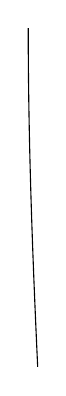
\begin{tikzpicture}\draw[thin] (0,0) .. controls (0,-1.5) and (0.06,-3) .. (0.12,-4.3);\end{tikzpicture}}}
\uline{Conséquence conjecturale} Soit $\Gamma'\subset\operatorname{Im}(\mathcal E_U\longrightarrow\Gamma_{\mathbb{Q}}\unsure{)}$ un sous-groupe ouvert, correspondant à un corps $k$ fini sur $\mathbb{Q}$, considérons un $k$-point de $U$, d'où un relèvement $\Gamma'\unsure{-|\longrightarrow}\mathcal E_U$, de sorte que $\Gamma'$ opère sur $\unsure{\Pi|\pi}_{\unsure{U|K}}$. Ceci posé\unsure{,} on a
\[
\unsure{\Pi|\pi}_U^{\Gamma'^\circ}=\{1\}.
\]

On étudiera par la suite les relations entre cette \unsure{``}\inserted{cons.} conjecturale'', et la précédente (d'apparence opposée !) concernant les $\mathcal E_K$.

La conjecture fondamentale, sur les modèles implique la conjecture fondamentale sur les corps, à condition de prendre soin, dans cette dernière, de se limiter aux hom compatibles aux filtrations modéliques,
\margin{et il vaut mieux se borner à l'\unsure{équivt.|équiv.} de a) et b) -- \unsure{la|les} \unsure{condition|conditions} c) sur les centralisateurs \unsure{risquent|risque} de passer mal à la $\varprojlim$}

Plus généralement, prenant \inserted{\unsure{complets|complètes|compacts} pour $U$} des schémas, \deleted{\unsure{de dim}} qui sont des $\varprojlim$ de \deleted{\unsure{schémas}} \inserted{modèles élém.} \unsure{anabéliques|anabéliens}, avec morphismes de transition \inserted{des imm ouvertes} affines
\margin{48}
